\chapter{CDP, LLDP, NTP, and Syslog}

\section{CDP}

Cisco Discovery Protocol (CDP) is a Cisco proprietary Layer 2 protocol that gathers information about Cisco devices sharing the same data link. CDP can also be used as a network discovery tool to determine the information about the neighboring devices. \\

CDP is disabled globally for all interfaces using the \verb|no cdp run| command. To enable CDP globally for all the supported interfaces on the device, enter \verb|cdp run| in the global configuration mode. The \verb|show cdp| command verifies the status and displays information about CDP.\\

To disable CDP on specific interfaces before enable CDP. For example, Branch-Edge has two active interface s0/0/1 and g0/0. To turn on CDP, first disable CDP on the s0/0/1 interface and then turn on the CDP protocol.

\begin{verbatim}
Branch-Edge# configure terminal
Branch-Edge(config)# interface s0/0/1
Branch-Edge(config-if)# no cdp enable
Branch-Edge(config-if)# exit
Branch-Edge(config)# cdp run
\end{verbatim}

Use \verb|show cdp| command to check if CDP is running. Use \verb|show cdp interface| to display the interfaces that are CDP enabled on a device. \\

\begin{figure}[hbtp]
\caption{Discovering Device Connected to S1}\label{CDP}
\centering
\subfigure[Output of show command]{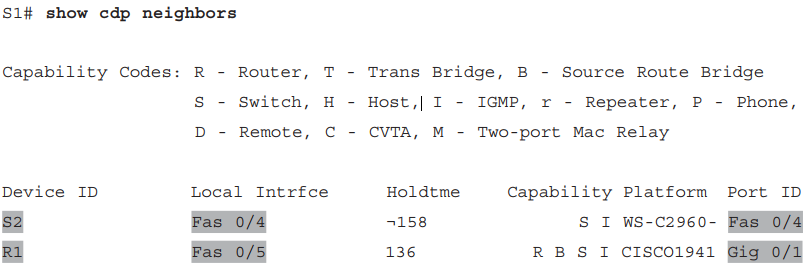
\includegraphics[ width=0.4\textwidth ]{pictures/CDP.PNG}}
\subfigure[Topology]{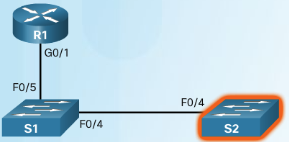
\includegraphics[ width=0.4\textwidth ]{pictures/CDPdiscover.PNG} }
\end{figure}

With CDP enabled on the network, the \verb|show cdp neighbors| and \verb|show cdp neighbors detail| command can be used to determine the network layout (Figure \ref{CDP}).

\section{LLDP}

LLDP (Link Layer Discovery Protocol) is a vendor-neutral neighbor discovery protocol similar to CDP. To enable LLDP globally on a Cisco network device, enter the \verb|lldp run| global configuration command. To disable LLDP, enter the \verb|no lldp run| command in the global configuration mode. Similar to CDP, LLDP can be configured on specific interfaces. However, LLDP must be configured separately to transmit and receive LLDP packets:

\begin{verbatim}
S1(config)# lldp run
S1(config)#
S1(config)# interface gigabitethernet 0/1
S1(config-if)# lldp transmit
S1(config-if)# lldp receive
S1(config-if)# end
S1#
S1# show lldp
S1# show lldp neighbors
S1# show lldp neighbors detail 
\end{verbatim}

\section{NTP}

\subsection{System clock}

The software clock on a router or switch starts when the system boots and is the primary source of time for the system. It is important to synchronize the time across all devices on the network because all aspects of managing, securing, troubleshooting, and planning networks require accurate time-stamping. \\

Typically, the date and time settings on a router or switch can be set using one of two methods: 

\begin{itemize}
\item Manually configure the date and time. For example, \verb|clock set 20:36:00 aug 30 2016|
\item Configure the NTP
\end{itemize}

\subsection{NTP operation}

NTP allows routers on the network to synchronize their time settings with an NTP server. It uses UDP port 123. \\

NTP networks use a hierarchical system of time sources. Each level in this hierarchical system is called a stratum. The stratum level is defined as the number of hop counts from the authoritative time source (Figure \ref{NTP}). Smaller stratum numbers indicate that the server is closer to the authorized time source than larger stratum numbers. The max hop count is 15. Stratum 16, the lowest stratum level, indicates that a device is unsynchronized. 

\begin{figure}[hbtp]
\caption{NTP Stratum levels}\label{NTP}
\centering
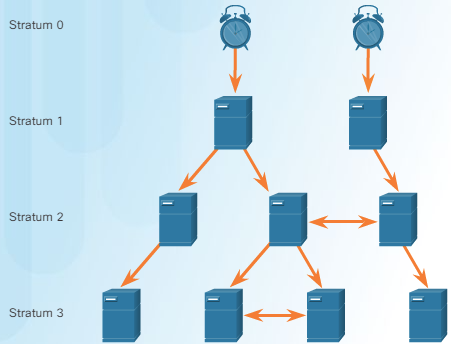
\includegraphics[ scale=0.6 ]{pictures/NTP.PNG}
\end{figure}

\paragraph{Stratum 0} An NTP network gets the time from authoritative time sources. Stratum 0 devices are represented by the clock in the figure \ref{NTP}.

\paragraph{Stratum 1} are directly connected to the authoritative time sources. They act as the primary network time standard.

\paragraph{Stratum 2 and Lower}The stratum 2 servers are connected to stratum 1 devices through network connections. Stratum 2 devices, such as NTP clients, synchronize their time using the NTP packets from stratum 1 servers. They can also act as servers for stratum 3 devices.

\subsection{Configure and Verify NTP}

To verify the system clock, use \verb|show clock [detail]| command. To identify NTP server, use \verb|ntp server <ip-addr>|. To see if the device is synchronized with the NTP server, use \verb|show ip ntp associations| and \verb|show ntp status|.

\section{Syslog}

\subsection{Introduction}

The syslog protocol allows networking devices to send their system messages across the network to syslog servers. The syslog server serves as an event message collector. Syslog messages are sent using UDP port 514. The syslog logging service provides three primary functions:

\begin{itemize}
\item Gather logging information
\item Select the type of logging information
\item Specify the destination of captured syslog messages
\end{itemize}

Syslog messages may be sent to an internal buffer. Messages sent to the internal buffer (RAM) are only viewable through the CLI of the device (console line, terminal line). Alternatively, syslog messages may be sent across the network to an external syslog server.\\

To view syslog messages, a syslog server must be installed on a workstation. One advantage of viewing syslog messages on a syslog server is the ability to perform granular searches through the data. Also, a network administrator can quickly delete unimportant syslog messages from the database.

\subsection{Severity level and Facility}
Cisco devices produce syslog messages as a result of network events. Every syslog message contains a \textbf{severity level} and a \textbf{facility}. The security level can be shown as a number. The smaller the number, the more critical syslog alarms (Table \ref{tab:Syslog}).\\

\begin{table}[hbtp]
\centering\caption{Syslog Severity level}\label{tab:Syslog}
\begin{tabular}{cc p{10cm} }
\toprule
\head{Severity level} & \head{Name} & \head{Explanation}\\

0 & Emergency & A "panic" condition, System unusable \\
1 & Alert & Should be corrected immediately, e.g. loss of backup ISP connection \\
2 & Critical & Critical condition \\
3 & Error & Error condition, Non-urgent failures \\
4 & Warning & NOT an error, but indication that an error will occur if action is not taken, e.g. file system 85\% full \\
5 & Notification & Normal but significant condition \\
6 & Informational & Not affect functionality, harvested for reporting, measuring throughput,\\
7 & Debugging & Debugging message \\
\bottomrule
\end{tabular}
\end{table}

Level 0 -- 4 are error messages. Level 5 notifies system messages such as interface up or down transitions and system restart messages. Level 6 generates messages , for example, when the device is booting. \\

By default, Cisco routers and switches send log messages for all severity (levels Level 0 through 7) to the console. \\

The facility represents the machine process that created the syslog event. For example, is the event created by the kernel, by the mail system, by security/authorization processes, etc.? The Facility value is a way of determining which process of the machine created the message. \\

\subsection{Message format}

By default, the format of syslog messages on the Cisco IOS Software is as follows:

\begin{verbatim}
seq no: timestamp: %facility-severity-MNEMONIC: description
00:00:46: %LINK-3-UPDOWN: Interface Port-channel1, changed state to up
\end{verbatim}

The fields contained in the syslog message above are explained in Table \ref{tab:SyslogFormat}.

\begin{table}[hbtp]
\centering\caption{Syslog message format}\label{tab:SyslogFormat}
\begin{tabular}{ll p{12cm} }
\toprule
\head{Field} & \head{Example} &\head{Explanation}\\
\midrule

\verb|seq no| & -- & Will be shown only if the \verb|service sequence-numbers| global configuration command is configured \\

\verb|timestamp| & \verb|00:00:46| & Date and time of the message, which appears only if the service timestamps global configuration command is configured \\

\verb|facility| & \verb|LINK| &The facility to which the message refers \\

\verb|severity| &  \verb|3| &A number from 0 to 7  that indicates the severity of the message \\

\verb|MNEMONIC| & \verb|UPDOWN| & Briefly and Uniquely describe the message\\

\verb|description| & \verb|Interface ...| & Report the event in detail\\

\bottomrule
\end{tabular}
\end{table}


\subsection{Configuration}

By default, log messages do not include a timestamp. To enable timestamp, use the following command

\begin{verbatim}
R1(config)# service timestamps log datetime
\end{verbatim}

The \verb|show logging| command displays the default logging service settings.\\

There are three steps to configuring the router to send system messages to a syslog server:

\begin{enumerate}
\item Use \verb|logging <ip-addr>| to configure IP address of the syslog server

\item Use the \verb|logging trap <level>| to configure severity level. For example, to limit the messages to levels 4 and lower (0 to 4), use the \verb|logging trap 4 | command. This sends Level 0 through 4 severity messages.

\item (Optional) Configure the source interface with the \verb|logging source <int>| command. This specifies that syslog packets contain the IP address of a specific interface, regardless of which interface the packet uses to exit the router.
\end{enumerate}

\begin{verbatim}
R1(config)# logging 192.168.1.3
R1(config)# logging trap 4
R1(config)# logging source-interface GigabitEthernet 0/0
R1(config)# interface loopback 0
\end{verbatim}

In this example, R1 is configured to send log messages of levels 4 and lower to the syslog server at 192.168.1.3. The source interface is set as the G0/0 interface. A loopback interface is created, shut down, and then brought back up. The console output reflects these actions.